\documentclass[11pt]{report}
\setcounter{secnumdepth}{3}
\setlength{\textwidth}{6.5in}
\setlength{\textheight}{9in}
\setlength{\oddsidemargin}{-0.0in}
\setlength{\evensidemargin}{-0.0in}
\setlength{\topmargin}{-0.5in}
\usepackage[utf8]{inputenc}
\usepackage[T1]{fontenc}
\input{def-logique}
\newcommand{\comment}[1]{}
\newcommand{\mfindex}[1]{#1\index{#1}}
\makeindex
\usepackage[totoc]{idxlayout}
\usepackage[nottoc]{tocbibind}
\usepackage{hyperref}
\usepackage{xspace}
\newcommand{\solution}[1]{\textbf{Solution:} #1}
\newcommand{\md}[1]{\textsf{#1}}
%\newcommand{\solution}[1]{}

\begin{document}
\begin{center}
Université	de	Sherbrooke	- Département	d'informatique\\
IGL501-IGL710 - Méthodes formelles en génie logiciel \\
Marc	Frappier,	professeur\\
\end{center}

\begin{center}
\Large\bf L'exemple de la pharmacie (version complexe)
\end{center}

Le système doit gérer les prescriptions effectuées pour des patients.  Certains patients sont allergiques à certains médicaments. Il faut donc que le système empêche la prescription de ces médicaments à un patient. On peut prescrire plusieurs médicaments en même temps à un patient. Certains médicaments sont incompatibles et ils ne peuvent être prescrits en même temps à un patient.  Certains médicaments ne peuvent être prescrits qu’à un seul des deux sexes biologiques. L’association \md{restriction} indique, le cas échéant, à quel sexe le médicament est restreint. Si un médicament n’est pas restreint à un seul des deux sexes, alors il n’est pas associé à un sexe dans la base de données.  Certains patients ont les caractéristiques des deux sexes biologiques. Dans ce cas, un médicament restreint à un seul sexe biologique ne peut leur être prescrit.  Finalement, certains médicaments nécessitent un âge minimal pour être prescrit à un patient. Si l'âge du patient n'est pas connu, alors on ne peut pas lui prescrire un médicament avec un age minimal.

L’attribut \md{idPatient} permet d’identifier de manière unique un patient.  L’attribut \md{idRAMQ} permet aussi d’identifier de manière unique un patient.  L’attribut \md{âge} est facultatif pour un patient.

L’attribut \md{idMedic} permet d’identifier de manière unique un médicament.  L’attribut \md{DIN} permet aussi d’identifier de manière unique un médicament, mais certains médicaments n’en ont pas.  L’attribut \md{description} doit être unique pour un médicament.

La figure~\ref{fig-ER} représente le diagramme entité-association de ce système.
\begin{figure}[b]
\begin{center}
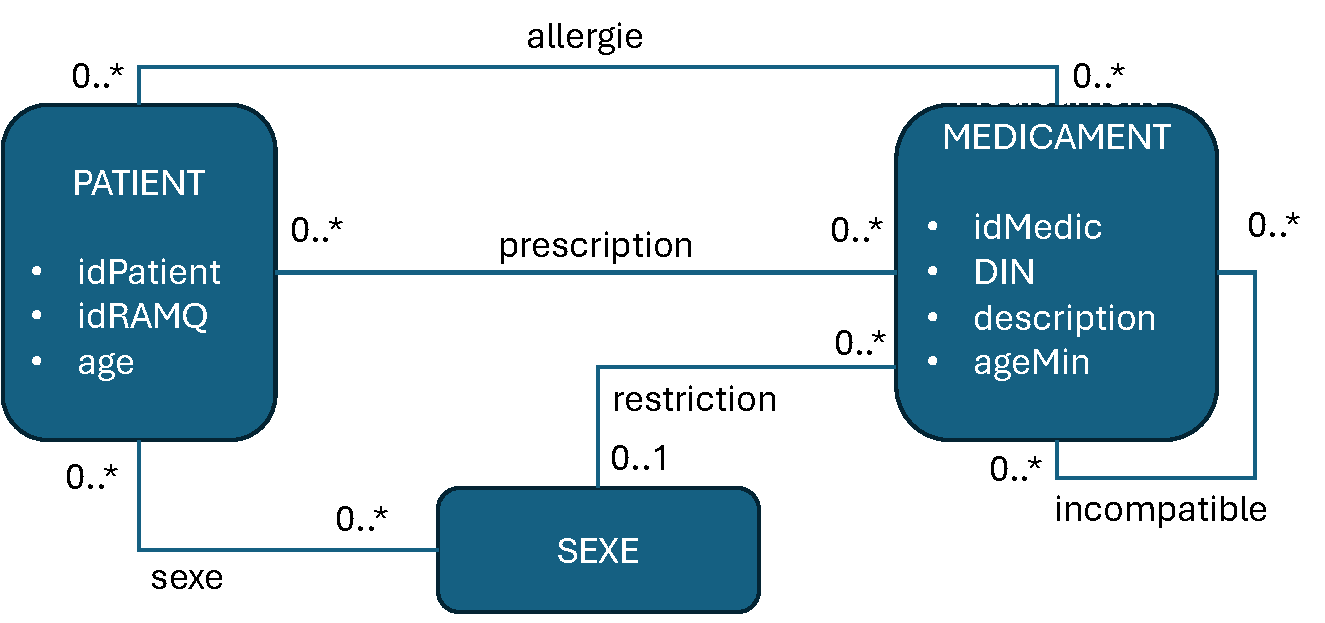
\includegraphics[scale=0.65]{pharmacie-ER.pdf}
\end{center}
\caption{Diagramme entité-association du système de gestion d'une pharmacie}
\label{fig-ER}
\end{figure}

\end{document}